% !TeX program = xelatex
% !TeX encoding = UTF-8
% Báo cáo dựa trên source add5f32 và kiểm thử ngày 11/11/2026.
\documentclass[11pt,a4paper]{article}
\usepackage[margin=20mm,top=19mm,bottom=19mm,headheight=14pt,headsep=7mm,footskip=10mm]{geometry}
\usepackage{fontspec}
\setmainfont{Times New Roman}
\setsansfont{Arial}
\setmonofont[Scale=0.88]{Consolas}
\usepackage{amsmath,amssymb,graphicx,xcolor,booktabs,tabularx,array,enumitem}
\usepackage{tikz}
\usetikzlibrary{arrows.meta,positioning,calc,shapes.geometric}
\usepackage{fancyhdr,titlesec,microtype}
\usepackage[unicode,colorlinks=true,linkcolor=navy,urlcolor=teal,citecolor=navy]{hyperref}
\definecolor{navy}{HTML}{17364D}
\definecolor{teal}{HTML}{007F83}
\definecolor{pale}{HTML}{EDF4F7}
\definecolor{ink}{HTML}{24313B}
\definecolor{muted}{HTML}{52636F}
\definecolor{linegray}{HTML}{D8E1E7}
\color{ink}
\pagestyle{fancy}
\fancyhf{}
\fancyhead[L]{\sffamily\small\textbf{CHAT CHAIN}\quad /\quad BLOCKCHAIN LAB 01}
\fancyhead[R]{\sffamily\small Báo cáo dự án}
\fancyfoot[L]{\sffamily\footnotesize Phiên bản mã nguồn: \texttt{add5f32}}
\fancyfoot[R]{\sffamily\footnotesize\thepage\,/\,\pageref{report:last}}
\renewcommand{\headrulewidth}{0.4pt}
\renewcommand{\footrulewidth}{0pt}
\titleformat{\section}{\Large\sffamily\bfseries\color{navy}}{\thesection.}{0.5em}{}
\titleformat{\subsection}{\normalsize\sffamily\bfseries\color{teal}}{\thesubsection}{0.5em}{}
\titlespacing*{\section}{0pt}{0pt}{9pt}
\titlespacing*{\subsection}{0pt}{9pt}{4pt}
\setlength{\parindent}{0pt}
\setlength{\parskip}{5pt}
\setlength{\tabcolsep}{5pt}
\renewcommand{\arraystretch}{1.15}
\setlist[itemize]{leftmargin=4.5mm,itemsep=2pt,topsep=3pt,parsep=0pt}
\setlist[enumerate]{leftmargin=6mm,itemsep=3pt,topsep=3pt,parsep=0pt}
\newcolumntype{Y}{>{\raggedright\arraybackslash}X}
\newcolumntype{P}[1]{>{\raggedright\arraybackslash}p{#1}}
\newcommand{\code}[1]{\texttt{\detokenize{#1}}}
\newcommand{\key}[1]{\textbf{\color{navy}#1}}
\newcommand{\note}[1]{\par\smallskip\noindent\colorbox{pale}{\parbox{\dimexpr\linewidth-2\fboxsep\relax}{\small #1}}\par\smallskip}
\newcommand{\figcap}[1]{{\small\color{muted}\textit{#1}}\par}
\newcommand{\nextpage}{\clearpage}
\emergencystretch=2em
\renewcommand{\contentsname}{Mục lục}
\setcounter{tocdepth}{1}
% Thông tin định danh do nhóm cung cấp cho báo cáo Lab 01.
\newcommand{\TeamOneName}{Lâm Hoàng Vũ}
\newcommand{\TeamOneId}{23122056}
\newcommand{\TeamTwoName}{Lê Thái Ngọc}
\newcommand{\TeamTwoId}{23122012}
\newcommand{\TeamThreeName}{Lê Hải Đăng}
\newcommand{\TeamThreeId}{23122005}

\hypersetup{pdftitle={Chat Chain - Báo cáo Blockchain và ứng dụng - Lab 01},pdfauthor={Lê Hải Đăng; Lê Thái Ngọc; Lâm Hoàng Vũ},pdfsubject={Blockchain Layer 1 mô phỏng, đồng thuận BFT và kiểm thử xác định}}

\begin{document}
\hypersetup{pageanchor=false}
% Bìa không đánh số; thông tin môn học và giảng viên do nhóm cung cấp.
\begin{titlepage}
\thispagestyle{empty}
\begin{tikzpicture}[remember picture,overlay]
\draw[navy,line width=1.2pt]
  ($(current page.north west)+(15mm,-15mm)$)
  rectangle ($(current page.south east)+(-15mm,15mm)$);
\draw[navy,line width=0.35pt]
  ($(current page.north west)+(17mm,-17mm)$)
  rectangle ($(current page.south east)+(-17mm,17mm)$);
\end{tikzpicture}
\centering
\vspace*{8mm}
{\fontsize{13}{18}\selectfont
ĐẠI HỌC QUỐC GIA THÀNH PHỐ HỒ CHÍ MINH\par
\textbf{TRƯỜNG ĐẠI HỌC KHOA HỌC TỰ NHIÊN}\par
\textbf{KHOA CÔNG NGHỆ THÔNG TIN}\par}
\vspace{6mm}
{\color{navy}\rule{42mm}{0.6pt}\par}
\vspace{15mm}
{\large MÔN HỌC\par}
\vspace{2mm}
{\LARGE\bfseries Blockchain và ứng dụng\par}
\vspace{15mm}
{\Large\bfseries BÁO CÁO BÀI THỰC HÀNH 01\par}
\vspace{8mm}
{\fontsize{32}{38}\selectfont\bfseries\color{navy} CHAT CHAIN\par}
\vspace{4mm}
{\large Thiết kế và hiện thực Blockchain Layer 1\par
trên mạng mô phỏng không tin cậy\par}
\vspace{15mm}
{\large Giảng viên hướng dẫn: \textbf{Ngô Đình Hy}\par}
\vspace{12mm}
{\large\bfseries Sinh viên thực hiện\par}
\vspace{4mm}
{\large\renewcommand{\arraystretch}{1.45}
\begin{tabular}{@{}l@{\hspace{18mm}}l@{}}
\textbf{Họ và tên} & \textbf{MSSV}\\
\TeamThreeName & \TeamThreeId\\
\TeamTwoName & \TeamTwoId\\
\TeamOneName & \TeamOneId\\
\end{tabular}\par}
\vfill
{\large Thành phố Hồ Chí Minh, tháng 11 năm 2026\par}
\vspace*{7mm}
\end{titlepage}

\hypersetup{pageanchor=true}
\pagenumbering{roman}
% Mục lục dùng số La Mã, tách khỏi phần nội dung đánh số Ả Rập.
\thispagestyle{plain}
\tableofcontents
\vspace{8mm}
\subsection*{Tóm tắt}
Chat Chain mô phỏng một kênh chat chung: mỗi tin nhắn là giao dịch có chữ ký, các validator thống nhất thứ tự bằng quy trình đề xuất, prevote, precommit và finalize. Dự án sử dụng 10 validator, chịu tối đa 3 lỗi Byzantine theo giả định của bài, chạy trong một process với đồng hồ ảo và nguồn ngẫu nhiên theo seed. Mỗi node giữ state, ledger và view riêng; mọi trao đổi giữa node đi qua mạng mô phỏng.

Báo cáo đối chiếu đề \code{Lab01.pdf}, mã nguồn tại commit \code{add5f32} và lần chạy kiểm thử ngày \textbf{11/11/2026}. Các giới hạn và sai khác so với README được nêu ở Mục 8.

\vspace{4mm}
\subsection*{Phân công thực hiện}
{\small
\begin{tabularx}{\linewidth}{P{37mm}P{22mm}Y}
\toprule
\textbf{Họ và tên} & \textbf{MSSV} & \textbf{Phần việc chính}\\
\midrule
\TeamThreeName & \TeamThreeId & Consensus, Node orchestration, block builder, view, vote counter và kiểm thử e2e.\\
\TeamTwoName & \TeamTwoId & Mật mã, dữ liệu lõi, thực thi state, validation, pool, ledger, sync và query.\\
\TeamOneName & \TeamOneId & Đồng hồ ảo, mạng, gossip, log, fault hooks, cấu hình và tích hợp môi trường.\\
\bottomrule
\end{tabularx}\par}
\vfill
{\small Kho mã nguồn: \url{https://github.com/CatnCactus72/Blockchain_lab01}\par}

\clearpage
\pagenumbering{arabic}
\pagestyle{fancy}
\section{Giới thiệu và cấu trúc dự án}
\subsection{Mục tiêu và quyết định thiết kế}
Mục tiêu là duy trì một lịch sử tin nhắn đã finalize nhất quán khi gói tin có thể trễ, trùng, đảo thứ tự hoặc mất trước GST. Ứng dụng chọn phép ghi \code{SET} vào không gian tên của người gửi, không có gas, phí hay thực thi song song. Thứ tự chat lấy từ ledger theo height và vị trí giao dịch trong block, không lấy từ thứ tự duyệt state.

\begin{itemize}
\item \key{BFT với tập validator cố định:} $n=3f+1=10$, $f=3$, quorum $q=2f+1=7$. Lịch proposer xác định theo height và round, không có một node điều phối trung tâm.
\item \key{Header trước, body sau:} proposal mang header; body chỉ tải qua yêu cầu trực tiếp sau kiểm tra header. Cách này tách xác nhận thông tin đề xuất khỏi truyền tải danh sách giao dịch.
\item \key{Xác thực và cam kết:} Ed25519 cho chữ ký, SHA-256 cho định danh/cam kết; state hash là hash phẳng của map chuẩn hóa, không dùng cây Merkle.
\item \key{Tái lập:} đồng hồ ảo, queue có tie-break và RNG con theo thành phần giúp phân biệt lỗi giao thức với nhiễu do môi trường chạy.
\end{itemize}

\subsection{Kiến trúc và ranh giới module}
\begin{center}
\begin{tikzpicture}[x=1cm,y=1cm,box/.style={draw=linegray,fill=pale,rounded corners=2pt,minimum height=12mm,text width=40mm,align=center,font=\sffamily\small},arr/.style={-{Latex[length=2mm]},thick,color=teal},lab/.style={font=\scriptsize,fill=white,inner sep=1pt}]
\node[box] (cfg) at (0,3) {\textbf{CLI + cấu hình}\\seed, topology, workload, faults};
\node[box] (sim) at (5,3) {\textbf{Simulator}\\Clock / Queue / RNG};
\node[box] (net) at (10,3) {\textbf{Network + Link}\\gossip / hạn mức / peer block};
\node[box] (core) at (0,0) {\textbf{Core / Crypto / Execution}\\đối tượng, chữ ký, state};
\node[box] (node) at (5,0) {\textbf{Node riêng cho N0--N9}\\Consensus / View / Pool / Sync};
\node[box] (log) at (10,0) {\textbf{Logsys + công cụ}\\event / summary / trace};
\draw[arr] (cfg)--(sim);
\draw[arr] (sim)--(net);
\draw[arr] (sim)--node[lab,left]{timer / callback}(node);
\draw[arr] (core)--(node);
\draw[arr,<->] (node.north east)--(net.south west);
\node[lab,align=center,text width=27mm] at (7.9,1.5) {NodeEnv\\send / receive};
\draw[arr] (node)--(log);
\draw[arr] (net)--(log);
\end{tikzpicture}
\end{center}
\figcap{Hình 1. Các module và đường tương tác chính. Node không import sim/net; transport không thực thi quy tắc BFT. Simulator điều phối thời gian, không quyết định block được finalize.}

{\small
\begin{tabularx}{\linewidth}{P{36mm}Y}
\toprule
\textbf{Thư mục / điểm vào} & \textbf{Trách nhiệm}\\\midrule
\code{src/sim}, \code{src/net} & Lập lịch sự kiện; topology; số phận gói; dedup; rate limiting.\\
\code{src/crypto}, \code{src/core} & Encoding, keybook, ký/xác minh, Transaction, Header, Block, Proposal, Vote, Message.\\
\code{src/execution} & State riêng và phép chuyển trạng thái xác định, có thực thi thử.\\
\code{src/node} & Node, consensus, proposer, builder, view, counter, validation, ledger, sync, query.\\
\code{src/faults}, \code{src/logsys} & Hook lỗi tách khỏi node trung thực; log và summary nhất quán.\\
\code{config}, \code{tests}, \code{logs} & Tham số/scenario; unit/e2e/invariants/công cụ; bằng chứng thực thi.\\
\code{src/main.py} & Nạp base + scenario, dựng mạng/node/workload, chạy và xuất kết quả.\\
\bottomrule
\end{tabularx}}

\nextpage
\section{Mô hình dữ liệu, mật mã và các guard}
\subsection{Từ giao dịch đến cam kết trạng thái}
Giao dịch có account, nonce, key, value và signature. Key đúng dạng \code{account/chat/nonce}; nonce bắt đầu từ 1. State lưu map key--value và nonce đã áp dụng. Block gồm header và danh sách transaction có thứ tự; header chứa chain ID, height, parent hash, tx root, state hash, proposer, timestamp và chữ ký.

Round nằm trong proposal/vote, không nằm trong block hash. Nhờ đó, một block đã khóa có thể được đề xuất lại ở round sau mà không thay danh tính block. Proposal giữ chữ ký header của người tạo và có chữ ký riêng của proposer round hiện tại.

\begin{align*}
\text{state\_hash} &= \operatorname{SHA256}\bigl(\operatorname{encStr}(\text{STATE})\,\Vert\,\operatorname{encMap}(S)\bigr),\\
\text{msg\_id} &= \operatorname{SHA256}\bigl(\operatorname{encStr}(\text{MSG})\,\Vert\,\operatorname{encStr}(k)\,\Vert\,\operatorname{encStr}(o)\,\Vert\,\operatorname{encPayload}(p)\bigr).
\end{align*}
Trong đó $k,o,p$ lần lượt là kind, origin và payload; $\Vert$ là phép nối byte. Hash không dựa trên JSON. Chuỗi được chuẩn hóa NFC rồi mã hóa UTF-8; số nguyên dùng 64 bit big-endian; bytes/string có tiền tố độ dài; map sắp theo byte khóa; NIL được mã hóa riêng. Giá trị $\text{pol\_round}=-1$ sử dụng biểu diễn 64 bit theo quy ước encoding của dự án.

\subsection{Chữ ký và domain separation}
Mọi thao tác ký/xác minh đi qua \code{src/crypto/signing.py}. Dữ liệu ký có tiền tố domain và chain ID; chữ ký sai được thử ở các domain khác để phân biệt \code{WRONG_DOMAIN} với \code{BAD_SIGNATURE}. Thư viện \emph{cryptography} cung cấp Ed25519; định dạng khóa/chữ ký theo giao diện Ed25519 \cite{crypto,rfc8032}.

{\small\begin{tabularx}{\linewidth}{P{24mm}Y}
\toprule\textbf{Domain} & \textbf{Nội dung được ràng buộc bởi chữ ký}\\\midrule
TX & Account, nonce, key và value của giao dịch.\\
HEADER & Height, parent hash, tx root, state hash, proposer ID, timestamp.\\
PROPOSAL & Height, round, block hash và pol\_round.\\
VOTE & Height, round, phase, block hash hoặc NIL, validator ID.\\
\bottomrule\end{tabularx}}

Khóa được suy ra xác định từ seed, role và ID để chạy lại được. Đây là \textbf{quy ước thử nghiệm}; seed công khai không phải nguồn bí mật hay cơ chế quản lý khóa cho mạng thật.

\subsection{Các lớp kiểm tra trước khi tin dữ liệu}
\begin{enumerate}
\item \key{Giao dịch:} account tồn tại; chữ ký/domain hợp lệ; đúng quyền sở hữu và dạng key; value không rỗng, tối đa 200 ký tự NFC và 1024 byte/tx; nonce chống replay. Pool có thể giữ nonce tương lai, nhưng chỉ nonce kế tiếp mới được thực thi.
\item \key{Header/proposal:} đúng chain, parent và height; đúng proposer của round; chữ ký header/proposal hợp lệ; timestamp lớn hơn cha; block hash và POL nhất quán.
\item \key{Body/block:} đối chiếu tx root, giới hạn tổng body 4096 byte, thực thi tuần tự trên state cha rồi so state hash. Bất kỳ giao dịch sai làm body bị từ chối.
\item \key{Vote/certificate:} xác minh chữ ký, phase và cửa sổ height; mỗi validator chỉ được tính một vote trong một slot; certificate phải có ít nhất 7 PRECOMMIT hợp lệ cho cùng block/height/round.
\end{enumerate}

\nextpage
\section{Mạng mô phỏng và luồng thông điệp}
\subsection{Topology, độ trễ và hạn mức}
Mặc định có N0--N9, node $i$ kết nối $i\pm1$ và $i\pm2$ modulo 10: 4 peer/node, 20 cạnh vô hướng. Liên kết gần có base delay 20--60 ms, liên kết xa 60--120 ms; jitter nguyên từ 0 đến $\lfloor\text{base}/5\rfloor$. Mỗi chiều liên kết có RNG con riêng.

Trước GST, cấu hình gốc cho drop 30\%, duplicate 15\% và extra delay tối đa 4000 ms. Sau GST, không drop do Link; delay từng lần truyền qua liên kết không vượt $\Delta=500$ ms. Cận này tính từ lúc transmit, \textbf{không bao gồm thời gian đợi rate limit hoặc bị peer block}.

Outbound đặt trước tối đa 300 slot/node/cửa sổ 1000 ms; phần dư được hoãn, log \code{DELAY reason=RATE_LIMIT}. Inbound dùng cửa sổ trượt 1000 ms theo từng peer; vượt 200 message thì chặn 3000 ms, có BLOCK/UNBLOCK. Vì vậy, ``Link không drop sau GST'' không đồng nghĩa mọi callback đều nhận tin trong 500 ms.

\subsection{Gossip và cơ chế header trước body sau}
\begin{center}
\begin{tikzpicture}[x=1cm,y=1cm,arr/.style={-{Latex[length=1.7mm]},thick,color=teal},actor/.style={font=\sffamily\small,align=center},msg/.style={font=\scriptsize,fill=white,inner sep=1pt}]
\foreach \x/\name in {0/Client,3.4/Node nhận TX,6.8/Proposer hoặc peer,10.7/Validator}{
 \node[actor] at (\x,0.35) {\name};
 \draw[dashed,color=linegray] (\x,0)--(\x,-5.1);
}
\draw[arr] (0,-0.35)--node[msg,above]{TX có chữ ký}(3.4,-0.35);
\draw[arr] (3.4,-0.95)--node[msg,above]{gossip TX sau ACCEPT}(6.8,-0.95);
\draw[arr] (6.8,-1.55)--node[msg,above]{PROPOSAL: header + chữ ký}(10.7,-1.55);
\draw[arr] (10.7,-2.15)--node[msg,above]{BODY\_REQUEST sau kiểm tra header}(6.8,-2.15);
\draw[arr] (6.8,-2.75)--node[msg,above]{BODY: danh sách giao dịch}(10.7,-2.75);
\draw[arr] (10.7,-3.4)--node[msg,above]{PREVOTE block hợp lệ hoặc NIL}(3.4,-3.4);
\draw[arr] (3.4,-4.05)--node[msg,above]{quorum prevote: LOCK + PRECOMMIT}(10.7,-4.05);
\node[draw=teal,fill=pale,rounded corners=2pt,font=\sffamily\small,align=center] at (8.6,-4.75) {$\geq 7$ PRECOMMIT cùng block\\kiểm certificate và FINALIZE};
\end{tikzpicture}
\end{center}
\figcap{Hình 2. Luồng logic ở một height. Các mũi tên gossip biểu diễn lan truyền qua peer, không phải broadcast vật lý một hop tới toàn mạng. BODY có thể được lấy từ peer chuyển tiếp header.}

Gossip chỉ áp dụng cho TX, PROPOSAL, PREVOTE, PRECOMMIT. Mỗi node giữ tập seen theo \textbf{msg\_id đầy đủ}; chỉ chuyển tiếp khi callback trả ACCEPT và loại peer nguồn. REJECT/IGNORE không được forward. STATUS, BODY và các GET/response là point-to-point.

Message giữ nguyên danh tính qua các hop; Envelope mang from/to/time của từng hop. Network tạo snapshot riêng khi gửi và khi gọi receiver, tránh dataclass/payload mutable khiến một node vô tình sửa gói đang chờ hoặc dữ liệu của node khác. Mạng không xác minh luật đồng thuận: kết quả ACCEPT/REJECT do node quyết định.

\nextpage
\section{Đồng thuận, khóa và finality}
\subsection{Máy trạng thái của một height}
Sau khi finalize height $h$, node đợi 1000 ms ảo trước round 0 ở $h+1$. Proposer được xác định bởi $(\text{height}+\text{round})\bmod n$. \code{Consensus} giữ height, round, step, locked\_value/round và valid\_value/round; \code{View} lưu proposal, header, body và vote đã nhận.

\begin{enumerate}
\item \key{Propose.} Proposer đề xuất lại valid\_value nếu có, giữ nguyên header/hash và gắn POL; nếu không, builder chọn transaction theo thứ tự đến và nonce, dừng ở giao dịch đầu tiên không vừa 4096 byte, thực thi thử và ký block mới.
\item \key{Nhận header/body.} Node xác minh proposal rồi yêu cầu body. Body hợp lệ được cache; thiếu body thì thử peer khác sau timer. Body không có header tương ứng không được dùng để prevote.
\item \key{Prevote.} Node ở bước PROPOSE chỉ chuyển sang PREVOTE một lần; block phải qua validation và thỏa điều kiện khóa. Không có proposal/body hợp lệ trước timeout thì prevote NIL.
\item \key{Lock và precommit.} Quorum 7 prevote cùng block không-NIL, đã có body hợp lệ, cho phép ghi valid\_value và khóa block ở round hiện tại, sau đó precommit block. Nếu không thể có block quorum, hoặc timeout phù hợp, node precommit NIL.
\item \key{Finalize.} Nhận 7 precommit cho cùng block ở một round bất kỳ của height hiện tại, node lấy body hợp lệ, dựng certificate và thực thi lại. Ledger chỉ append sau kiểm chứng; State được cập nhật, pool loại TX đã dùng, phát TX\_APPLIED/FINALIZE rồi sang height mới.
\item \key{Timeout/nhảy round.} Timeout round $r$ là $5000+2000r$ ms; timer mang height/round nên timer cũ bị bỏ. Thấy $f+1=4$ validator ở round cao hơn cho phép nhảy round. Hết precommit timeout mà chưa finalize thì đổi proposer ở round tiếp.
\end{enumerate}

\subsection{Bảo vệ vote và điều kiện đổi khóa}
VoteCounter quản lý slot $(\text{validator},h,r,\text{phase})$: giữ phiếu hợp lệ đầu tiên, bỏ trùng, ghi bằng chứng khi nội dung mâu thuẫn. Quorum không được tạo bằng cách đếm lặp cùng validator. State machine và step guards giới hạn việc bỏ phiếu của node trung thực.

Khi đã khóa block $B$, node không tùy ý đổi sang $B'$ chỉ vì nhận proposal mới. Proposal có POL phải được đối chiếu với quorum prevote đã quan sát ở round tương ứng; nếu chưa đủ vote thì chờ thêm hoặc timeout. Các luật \code{_rule_*} được đánh giá lặp đến ổn định, có cờ chống gọi đệ quy, để body/proposal/vote đến theo thứ tự khác nhau không làm mất một chuyển trạng thái đã đủ điều kiện.

\subsection{Lập luận an toàn và phạm vi kết luận}
Hai quorum kích thước 7 trên 10 validator giao nhau ít nhất $2\times7-10=4$ validator. Với tối đa 3 Byzantine, giao có ít nhất một validator trung thực. Đây là cơ sở cho finality khi kết hợp quy tắc không double-vote và quy tắc khóa/POL qua các round; \textbf{phép đếm giao quorum riêng lẻ không thay thế chứng minh toàn bộ thuật toán}.

Safety yêu cầu các chain đúng tương thích tiền tố, cùng height có cùng hash; liveness chỉ được kỳ vọng sau GST với proposer đúng và đủ điều kiện nhận tin/đổi round. Các bài e2e cung cấp bằng chứng thực nghiệm cho cấu hình đã chạy, không chứng minh cho mọi lịch Byzantine có thể có.

\nextpage
\section{Ghi chú hiện thực và lỗi đã xử lý}
\subsection{Các lỗi có ý nghĩa trong quá trình tích hợp}
{\small\begin{tabularx}{\linewidth}{P{33mm}Y Y}
\toprule\textbf{Vấn đề} & \textbf{Nguyên nhân / hệ quả} & \textbf{Cách xử lý trong phiên bản hiện tại}\\\midrule
RNG bị khởi tạo lại & Gọi cùng nhãn lại nhận số đầu tiên; mất trạng thái luồng. & Cache Random theo node/nhãn; child stream được suy ra bằng hash nhãn có mã hóa độ dài.\\
Wire ID sau tiêm lỗi & Sửa chữ ký/payload mà giữ ID cũ khiến gossip dedup sai. & Dùng ID từ canonical Core/Wire; sửa bản sao; callback rebuild bắt lỗi ID chưa cập nhật.\\
Chữ ký bị sửa hai lần & Hook tạo vote rồi on\_send cùng đảo một byte có thể phục hồi chữ ký gốc. & Chỉ tiêm bad signature tại outbound; cache một bản sửa cho mỗi ID và không sửa tiếp bản đã phát.\\
Message bọc Proposal & Chữ ký ngoài Message rỗng; Proposal dùng trường proposal\_sig thay vì trường signature của dataclass. & Đi vào payload; thay đúng trường thật, giữ nguyên đối tượng gốc.\\
Payload dùng chung & Các callback có thể thay nội dung mà node khác hoặc queue đang tham chiếu. & Deepcopy ở biên transport và callback; state/pool/ledger tạo riêng theo node.\\
Sync thiếu certificate & Giá trị None gây lỗi truy cập; zip hai danh sách khác độ dài có thể bỏ sót dữ liệu. & Từ chối dữ liệu thiếu/hỏng hoặc thiếu keybook trước áp dụng; kiểm tra đủ block/certificate.\\
Log Unicode và viewer & Logger escape giá trị; viewer chưa unquote và từng dựng certificate giả để tái tạo ledger. & Giải mã trường log; dùng LogLedgerView chỉ để quan sát, không hạ quorum của Ledger thật.\\
Tương thích runtime & F-string dùng nháy lồng cùng loại gây SyntaxError ở Python 3.11. & Dùng biến trung gian; giữ yêu cầu Python 3.10+; cú pháp được kiểm trên grammar 3.10.\\
\bottomrule\end{tabularx}}

\subsection{Tính xác định và log}
VirtualClock chỉ tăng; EventQueue sắp theo $(t,seq)$, seq phá hòa theo thứ tự tạo sự kiện. Heap giảm chi phí chọn sự kiện tiếp theo; mỗi luồng Random độc lập để số lần gọi ở một liên kết không làm đổi luồng khác \cite{heapq,random}.

Mỗi log line có thời gian ảo, seq tăng, node, ev, height và các field theo thứ tự cố định. Thời gian thật chỉ dùng đặt tên file; nội dung không chứa datetime hay đường dẫn tạm. Kiểm tra determinism so \textbf{byte của toàn bộ log} và final state hash, không chỉ so số lượng block.

\subsection{Đồng bộ và cập nhật state}
Mỗi 2000 ms, STATUS trao đổi height/hash. Node chậm yêu cầu GET\_BLOCKS và tự kiểm block cùng certificate từ BLOCKS; node kẹt có thể xin GET\_VOTES/VOTES. State chỉ thay sau validation và thực thi thành công; dùng replace\_from để giữ tham chiếu State mà SyncManager đang giữ, thay vì đổi sang một object khiến hai thành phần nhìn hai state khác nhau. Certificate thiếu hoặc chữ ký không hợp lệ không được dùng để sao chép ledger từ peer.

\nextpage
\section{Kiểm thử và kết quả mong đợi}
\subsection{Bộ kiểm thử chung}
Điểm vào \code{python -m tests.run_all} chạy unit, T1--T8 rồi X1/X2; trả exit code khác 0 khi có FAIL/ERROR. Tại phiên bản báo cáo có \textbf{85 unit tests + 32 kiểm tra T1--T8 + 10 kiểm tra X1/X2 = 127 tests}. Không tính các lần chạy lại scenario của T8 thành số test độc lập.

{\small\begin{tabularx}{\linewidth}{P{36mm}P{10mm}Y}
\toprule\textbf{Nhóm unit} & \textbf{Số} & \textbf{Điều được kiểm tra}\\\midrule
Crypto / State & 7 / 7 & Chữ ký, sai domain, encoding/hash xác định; quyền sở hữu, nonce, replay, state hash.\\
VoteCounter & 12 & Dedup/conflict; phân biệt phase/round/NIL; quorum đúng 7; certificate và nhảy round.\\
Block / giới hạn & 12 / 3 & Parent, proposer, root/hash, timestamp, certificate; giới hạn NFC/byte và chọn TX.\\
Môi trường & 27 & Queue, clock, child RNG, timer, gossip, link bound, rate limit, block/unblock, config.\\
Tích hợp Phần 1/2 & 17 & Message/chữ ký thật, isolation, sync/fixture, workload, log Unicode và NodeEnv.\\
\bottomrule\end{tabularx}}

\subsection{Các scenario bắt buộc và mở rộng}
{\small\begin{tabularx}{\linewidth}{P{9mm}P{47mm}Y}
\toprule\textbf{ID} & \textbf{Điều kiện} & \textbf{Kỳ vọng và tiêu chí quan sát}\\\midrule
T1 & GST=0, không lỗi. & 10 node đúng có cùng chain/state; heights 1--10; không REJECT.\\
T2 & Duplicate 20\%, thêm trễ; N4 replay/copies=3. & Các node đúng hội tụ; có DUP; nonce đúng thứ tự; không finalize mâu thuẫn. N4 bị loại khỏi tập đúng.\\
T3 & N3 luân phiên lỗi chữ ký/domain/tamper. & REJECT có BAD\_SIGNATURE và WRONG\_DOMAIN; node đúng hội tụ.\\
T4 & Workload phát lại TX Alice; N5 đề xuất TX đã áp dụng. & Có REPLAYED\_TX; nonce Alice được áp dụng không lặp; chain đúng hội tụ.\\
T5 & GST=30 s, drop 30\%, dup 15\%, extra delay đến 4 s trước GST. & Có DROP/DELAY trước GST; giữ safety và hội tụ sau GST trong lần chạy.\\
T6 & N1 là proposer $(h=1,r=0)$ nhưng im lặng. & TIMEOUT rồi NEW\_ROUND r=1; height 1 finalize ở round sau; chain tiếp tục.\\
T7 & N2, N5, N8 equivocate bằng khóa của chúng. & Phát hiện CONFLICTING\_VOTE; origin của xung đột thuộc node lỗi; chain đúng không phân nhánh.\\
T8 & T1 và T7: hai lần seed 42, một lần seed 43. & Seed 42 cho log byte-identical và cùng final state hash; seed 43 cho log khác.\\
X1 & Thêm 100 TX trong 1 s, tại vùng 5--6 s. & Hội tụ, nonce tăng đúng, không thấy block bị từ chối quá khổ; có nhiều TX\_APPLIED.\\
X2 & N6--N9 im lặng: 4 lỗi, vượt $f=3$. & Không có FINALIZE; chạy đến giới hạn thời gian; không ghi nhận phân nhánh.\\
\bottomrule\end{tabularx}}

\note{Các invariant kiểm tra chain cùng height/hash, tương thích tiền tố, nonce không áp dụng lặp và đúng thứ tự, log đúng định dạng/thời gian/seq/reason. Vote counting được kiểm trực tiếp bằng unit VoteCounter; kiểm tra log hiện chưa tái dựng đầy đủ toàn bộ tally.}

\nextpage
\section{Số liệu thực nghiệm và phân tích}
% Generated by report/build_results.py from saved evidence.
Lần chạy ngày 11/11/2026: \textbf{127/127 tests PASS}, không có FAIL/ERROR; 15 lượt mô phỏng gồm 9 scenario và 6 lượt phục vụ T8. Bảng dưới dùng seed 42, thời gian ảo từ summary, không phải thời gian CPU.

{\small\begin{tabular*}{\linewidth}{@{\extracolsep{\fill}}lrrrrrr}
\toprule
\textbf{Ca} & \textbf{Giây ảo} & \textbf{Node đúng} & \textbf{Height} & \textbf{TX tại N0} & \textbf{DROP} & \textbf{REJECT}\\\midrule
T1 & 15.153 & 10 & 10 & 28 & 0 & 0 \\
T2 & 19.739 & 9 & 10 & 37 & 0 & 0 \\
T3 & 26.611 & 9 & 10 & 37 & 0 & 623 \\
T4 & 20.615 & 9 & 10 & 39 & 0 & 10 \\
T5 & 51.464 & 10 & 10 & 101 & 1133 & 80 \\
T6 & 26.297 & 9 & 10 & 40 & 0 & 1 \\
T7 & 26.826 & 7 & 10 & 52 & 0 & 304 \\
X1 & 15.222 & 10 & 10 & 114 & 0 & 0 \\
X2 & 120.000 & 6 & 0 & 0 & 0 & 0 \\
\bottomrule\end{tabular*}}
\figcap{Bảng 1. Height cuối bằng nhau trên các node đúng; TX là số sự kiện TX\_APPLIED riêng tại N0. DROP/REJECT được đếm trên toàn log. T1--T7/X1 đều hội tụ ở height 10; X2 dừng ở 120 s với height 0.}

\begin{center}
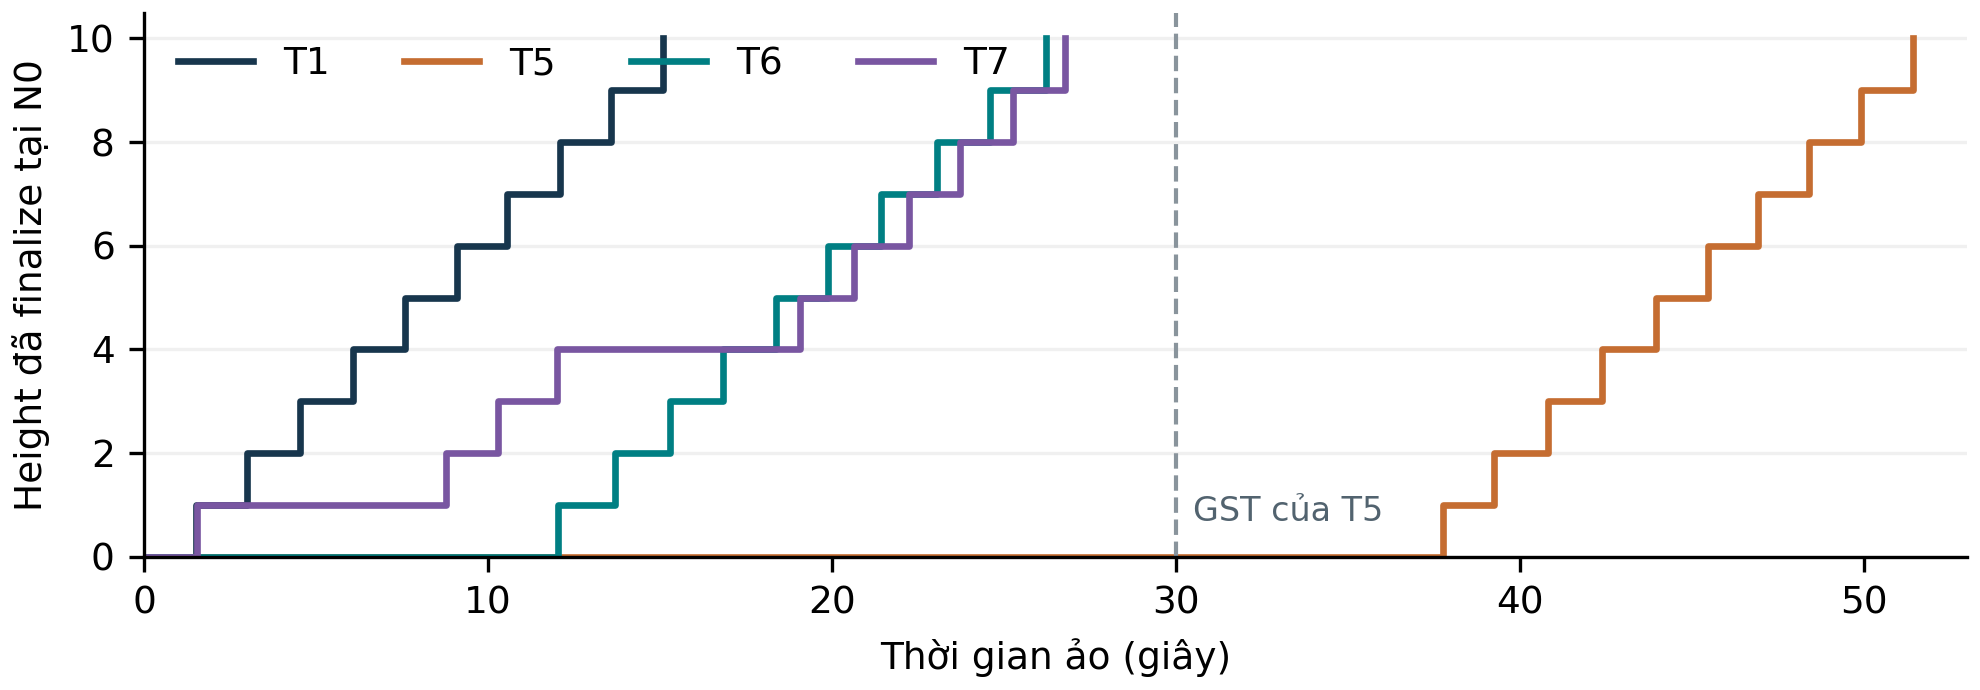
\includegraphics[width=0.94\linewidth]{report/figures/finalization.png}
\end{center}
\figcap{Hình 3. Tiến độ tại N0: T5 cần 51.464 s để toàn bộ node đúng đạt đích, so với 15.153 s ở T1. Đường nét đứt chỉ GST của T5; không phải một mốc của ba ca còn lại.}

{\small
\textbf{Quan sát lỗi:} T3 ghi 596 BAD\_SIGNATURE và 27 WRONG\_DOMAIN; T4 có 10 REPLAYED\_TX; T7 có 304 CONFLICTING\_VOTE. T5 có 1133 DROP và 80 DUPLICATE\_VOTE; T6 có 1 DUPLICATE\_VOTE. Các REJECT này phản ánh guard đang hoạt động, không phải test thất bại. T1 vẫn có 4232 DUP do cùng message đi tới node qua nhiều đường gossip, dù Link không tiêm lỗi duplicate. X1 áp dụng 114 TX tại N0; chưa kết luận mọi TX đã sinh đều được đưa vào chain.

\textbf{T8 -- tính xác định.} Hai log seed 42 trùng toàn bộ byte theo test, cùng final state hash; seed 43 cho log khác. Bảng 2 ghi 12 ký tự đầu SHA-256 để nhận diện; đối chiếu thực tế dùng digest đầy đủ và log gốc.

\begin{tabularx}{\linewidth}{lYYY}
\toprule
\textbf{Ca} & \textbf{Seed 42 / lần 1} & \textbf{Seed 42 / lần 2} & \textbf{Seed 43}\\\midrule
T1 & \code{e12ad6b6d06a} & \code{e12ad6b6d06a} & \code{549f197d3714} \\
T7 & \code{75f109db69da} & \code{75f109db69da} & \code{685c50883b3f} \\
\bottomrule\end{tabularx}
\par
}


\nextpage
\section{Thảo luận, giới hạn và tái lập}
\subsection{Phân biệt điều đã đạt và điều chưa được chứng minh}
\begin{itemize}
\item \key{Safety trong phạm vi chạy:} T1--T7/X1 không ghi nhận hai block khác nhau cùng height ở node đúng; T8 kiểm log và state thật. Đây là bằng chứng kiểm thử hữu hạn, chưa phải chứng minh giao thức với mọi seed, mọi tập Byzantine hoặc mọi lịch gói tin.
\item \key{An toàn khi vượt ngưỡng:} X2 có 6 validator hoạt động, không đủ quorum 7 nên không finalize. Các state rỗng bằng nhau có thể làm summary báo converged; điều này không đồng nghĩa có tiến triển hay đã đạt target height.
\item \key{T2 và node chậm:} node lỗi replay N4 có thể ở sau các node đúng. Kết luận hội tụ của summary chỉ áp dụng tập honest\_nodes, không buộc mọi node lỗi có cùng height.
\item \key{Giới hạn test X1:} test hiện đếm tổng TX\_APPLIED trên nhiều node và kiểm không có REJECT quá khổ. Nó chưa chứng minh mọi TX client đã sinh đều được finalize trước khi dừng ở height 10; cần bổ sung kiểm tra bằng tập tx\_id và kích thước từng block độc lập.
\item \key{Đếm vote và nonce:} helper vote\_counting\_problems chưa tái dựng tally từ log; unit VoteCounter mới là bằng chứng trực tiếp. Invariant nonce kiểm không lặp và thứ tự tăng, chưa thay thế được kiểm tra liên tục đầy đủ cho mọi log thiếu sự kiện.
\end{itemize}

\subsection{Sai khác đáng chú ý giữa README và hiện thực}
Workload \code{replay_alice} hiện phát lại TX Alice đầu tiên \textbf{một lần sau một nhịp 500 ms}, đổi origin/node nhận để không bị dedup wire che mất replay. Mô tả README rộng hơn: ba lần cách nhau 1 s và phát lại sau finalize. T4 hiện xác nhận chống replay và proposal chứa TX cũ, nhưng chưa bao phủ đúng toàn bộ lịch phát lại được mô tả đó.

Mode \code{bad_key} hiện đảo một byte chữ ký để sinh BAD\_SIGNATURE, không tạo một chữ ký hợp lệ bằng khóa khác. Với TX, node Byzantine không giữ khóa user nên nhánh wrong-domain dùng tamper thay thế; chữ ký WRONG\_DOMAIN thật được tạo trên vote/proposal do chính node lỗi sở hữu. Đây là giới hạn cần nêu rõ, không coi ba mode là ba mã reason khác nhau.

Topology mặc định có 10 node và 20 liên kết nhưng đọc từ file; đổi $n$ cần thay topology phù hợp. Khóa suy ra từ seed, một process và truyền object là cách tổ chức mô phỏng; không mô tả triển khai mạng P2P thực hay quản lý private key sản xuất. Chưa có fuzzing, chứng minh hình thức, benchmark nhiều seed hay kiểm thử n lớn trong báo cáo này.

\subsection{Cách chạy và điều kiện tái lập}
Môi trường kiểm tra là Windows, Python 3.11.8, \code{cryptography} 47.0.0, seed 42 và commit \code{add5f32}. Yêu cầu dự án là Python 3.10+; tương thích cú pháp không được coi là đã chạy mọi runtime.

\begin{quote}\small\ttfamily
python -m pip install -r requirements.txt\\
python -m tests.run\_all\\
python -m src.main --config config/scenarios/t1\_normal.json\\
python -m tests.check\_determinism --config config/scenarios/t7\_byzantine\_equivocate.json
\end{quote}
CLI hỗ trợ seed/faulty/out; \code{--smoke-env} chỉ là smoke hạ tầng. Log/summary thật và bằng chứng kiểm thử, thay vì nội dung smoke, là cơ sở cho phần kết quả trong báo cáo này.

\nextpage
\section{Tài liệu tham khảo và quy cách bàn giao}
\begin{thebibliography}{9}
\small
\bibitem{lab} Bộ môn Knowledge Engineering. \emph{Blockchain course 2026, Lab 01}, bản đề \code{Lab01.pdf} do môn học cung cấp, 5 trang. Các mục 3, 6--10 quy định fault model, locking, kiểm thử và báo cáo tối đa 10 trang.
\bibitem{repo} Nhóm Chat Chain. \emph{Blockchain\_lab01}, README, source và tests tại commit \code{add5f32}. \url{https://github.com/CatnCactus72/Blockchain_lab01}. Truy cập/đối chiếu local: 11/11/2026.
\bibitem{crypto} Python Cryptographic Authority. \emph{Ed25519 signing}. Tài liệu giao diện ký, xác minh và định dạng khóa/chữ ký của thư viện cryptography. \url{https://cryptography.io/en/latest/hazmat/primitives/asymmetric/ed25519/}. Truy cập: 11/11/2026; môi trường dự án dùng phiên bản 47.0.0.
\bibitem{rfc8032} S. Josefsson, I. Liusvaara. \emph{Edwards-Curve Digital Signature Algorithm (EdDSA)}. RFC 8032, 2017. \url{https://www.rfc-editor.org/rfc/rfc8032}.
\bibitem{heapq} Python Software Foundation. \emph{heapq -- Heap queue algorithm}, tài liệu Python 3.11. \url{https://docs.python.org/3.11/library/heapq.html}. Truy cập: 11/11/2026.
\bibitem{random} Python Software Foundation. \emph{random -- Generate pseudo-random numbers}, tài liệu Python 3.11. \url{https://docs.python.org/3.11/library/random.html}. Truy cập: 11/11/2026. RNG của simulator dùng để tái lập, không thay nguồn ngẫu nhiên mật mã.
\end{thebibliography}

\subsection*{Tài liệu nội bộ và công cụ}
\code{PERSON2_SUMMARY.md} mô tả API luật chuỗi. Lịch sử ghép phần 1/2 nằm trong \code{INTEGRATION_HANDOFF.md} và \code{PART1_PART2_INTEGRATION_REPORT.md}. Những đoạn PENDING trong tài liệu bàn giao cũ là trạng thái trước khi consensus được thêm, không thay kết quả kiểm thử hiện tại.

Báo cáo soạn bằng XeLaTeX, xem bằng LaTeX Workshop trong VS Code; không chép mã nguồn vào báo cáo. Bìa tham khảo cách trình bày tên trường/khoa trong hướng dẫn mẫu LaTeX tại \href{https://www.fit.hcmus.edu.vn/vn/Default.aspx?tabid=1064}{trang biểu mẫu chính thức của Khoa CNTT}; đây không phải mẫu bắt buộc riêng cho Lab01. Số liệu tổng hợp và kết quả kiểm thử lưu ở \code{report/evidence}; log gốc của lần chạy lưu local ở \code{tmp/pdfs/report_evidence}.

\subsection*{Đóng gói theo Mục 10 của đề}
Thư mục nộp cần có \code{src/}, \code{tests/}, \code{logs/}, \code{config/}, \code{README.md} và \code{REPORT.pdf}. Tên thư mục và ZIP mang tiền tố Lab01 cùng MSSV thành viên; nhóm có 3 người cần dùng đúng quy ước số ID do môn học chấp nhận, không tự bổ sung hai MSSV không có trong nhóm.

\subsection*{Kết luận}
Chat Chain đã ghép đủ các lớp mật mã, truyền tin, thực thi và đồng thuận để chạy blockchain mô phỏng với 10 validator. Bộ kiểm thử bao phủ trường hợp bình thường, lỗi truyền tin, chữ ký sai, replay, proposer im lặng và equivocation; các số liệu cho thấy hội tụ ở node đúng trong các lần chạy đã kiểm tra và giữ trạng thái không phân nhánh khi mất quorum. Hướng hoàn thiện tập trung vào lịch replay đúng mô tả, kiểm tra độc lập độ đầy đủ TX/kích thước block và mở rộng kiểm thử nhiều seed/tập lỗi.

\label{report:last}
\end{document}
